% aws_4.tex - AWS EMR for Cloud Computing class (Spring 2015)
% Chanmann Lim - April 2015

\documentclass[a4paper]{article}

\usepackage[margin=1 in]{geometry}
\usepackage{listings}
\usepackage{graphicx}
\usepackage{float}
\usepackage{hyperref}
\usepackage{amsmath}

\begin{document}
\title{CS 7001-03: Homework 4: AWS-EMR}
\author{Chanmann Lim\\ 
	\texttt{cl9p8@mail.mail.missouri.edu}}
\date{April 30, 2015}
\maketitle

% ---------------------------------------- 1 ----------------------------------------
\paragraph{1. } By default there is one Master instance with "m3.xlarge" EC2 instance type created in the EMR cluster and the main jobs of the Master node is to assign Hadoop tasks to the \textbf{core} and \textbf{task} nodes and monitor their status and there are two Core instances are also created in the EMR cluster for processing Hadoop tasks and storing the data using the Hadoop Distributed File System (HDFS) and to S3 using EMR File System (EMRFS).


% ---------------------------------------- 2 ----------------------------------------
\paragraph{2. } List of the first and last word with the associated number of occurrences from each output part file\\
\begin{description}
\leftskip 0.4in
\parindent -0.4in
	\item[part-00000: ] abbate	\textbf{1}, zoology	\textbf{3}
	\item[part-00001: ] abacus	\textbf{3}, zvith	\textbf{1}
	\item[part-00002: ] a	\textbf{4215}, zenith	\textbf{2}
	\item[part-00003: ] abandon	\textbf{6}, zweite	\textbf{1}
	\item[part-00004: ] abbreviated	\textbf{1}, yolk	\textbf{1}
	\item[part-00005: ] abandons	\textbf{2}, zeitschrift	\textbf{1}
	\item[part-00006: ] ab	\textbf{1}, zwanzig	\textbf{1}
\end{description}

% ---------------------------------------- 3 ----------------------------------------
\paragraph{3. } AWS-EMR execution chart: \\
\begin{center}
  \begin{tabular}{ |c|c|c|c| }
    \hline
    Master & Cores & Output parts & Cluster ID \\ \hline
    1 & 2 & 7 & j{-}2397PQCL7GDP1 \\ \hline
    1 & 3 & 11 & j{-}1VDWF9AKANGPE \\ \hline
    1 & 4 & 15 & j{-}8OJYX2FVDGZW \\ \hline
    1 & 5 & 19 & j{-}2BBG0J0YBRKL1 \\ \hline
    1 & 6 & 23 & j{-}2ACHK4SU3NDIB \\ \hline
  \end{tabular}
\end{center}

The number of output part files increased linearly as the number core instances get large. The observations above show that
\begin{align}
  part\_files = 4 \times cores - 1
\end{align}

The more core instances initiated to handle the MapReduce tasks the more chunks can be split from the original input file for parallel processing. \\
 
% ---------------------------------------- 4 ----------------------------------------
\paragraph{4. } Screenshot of the clusters created with EMR:
\begin{figure}[H]
  \centering
    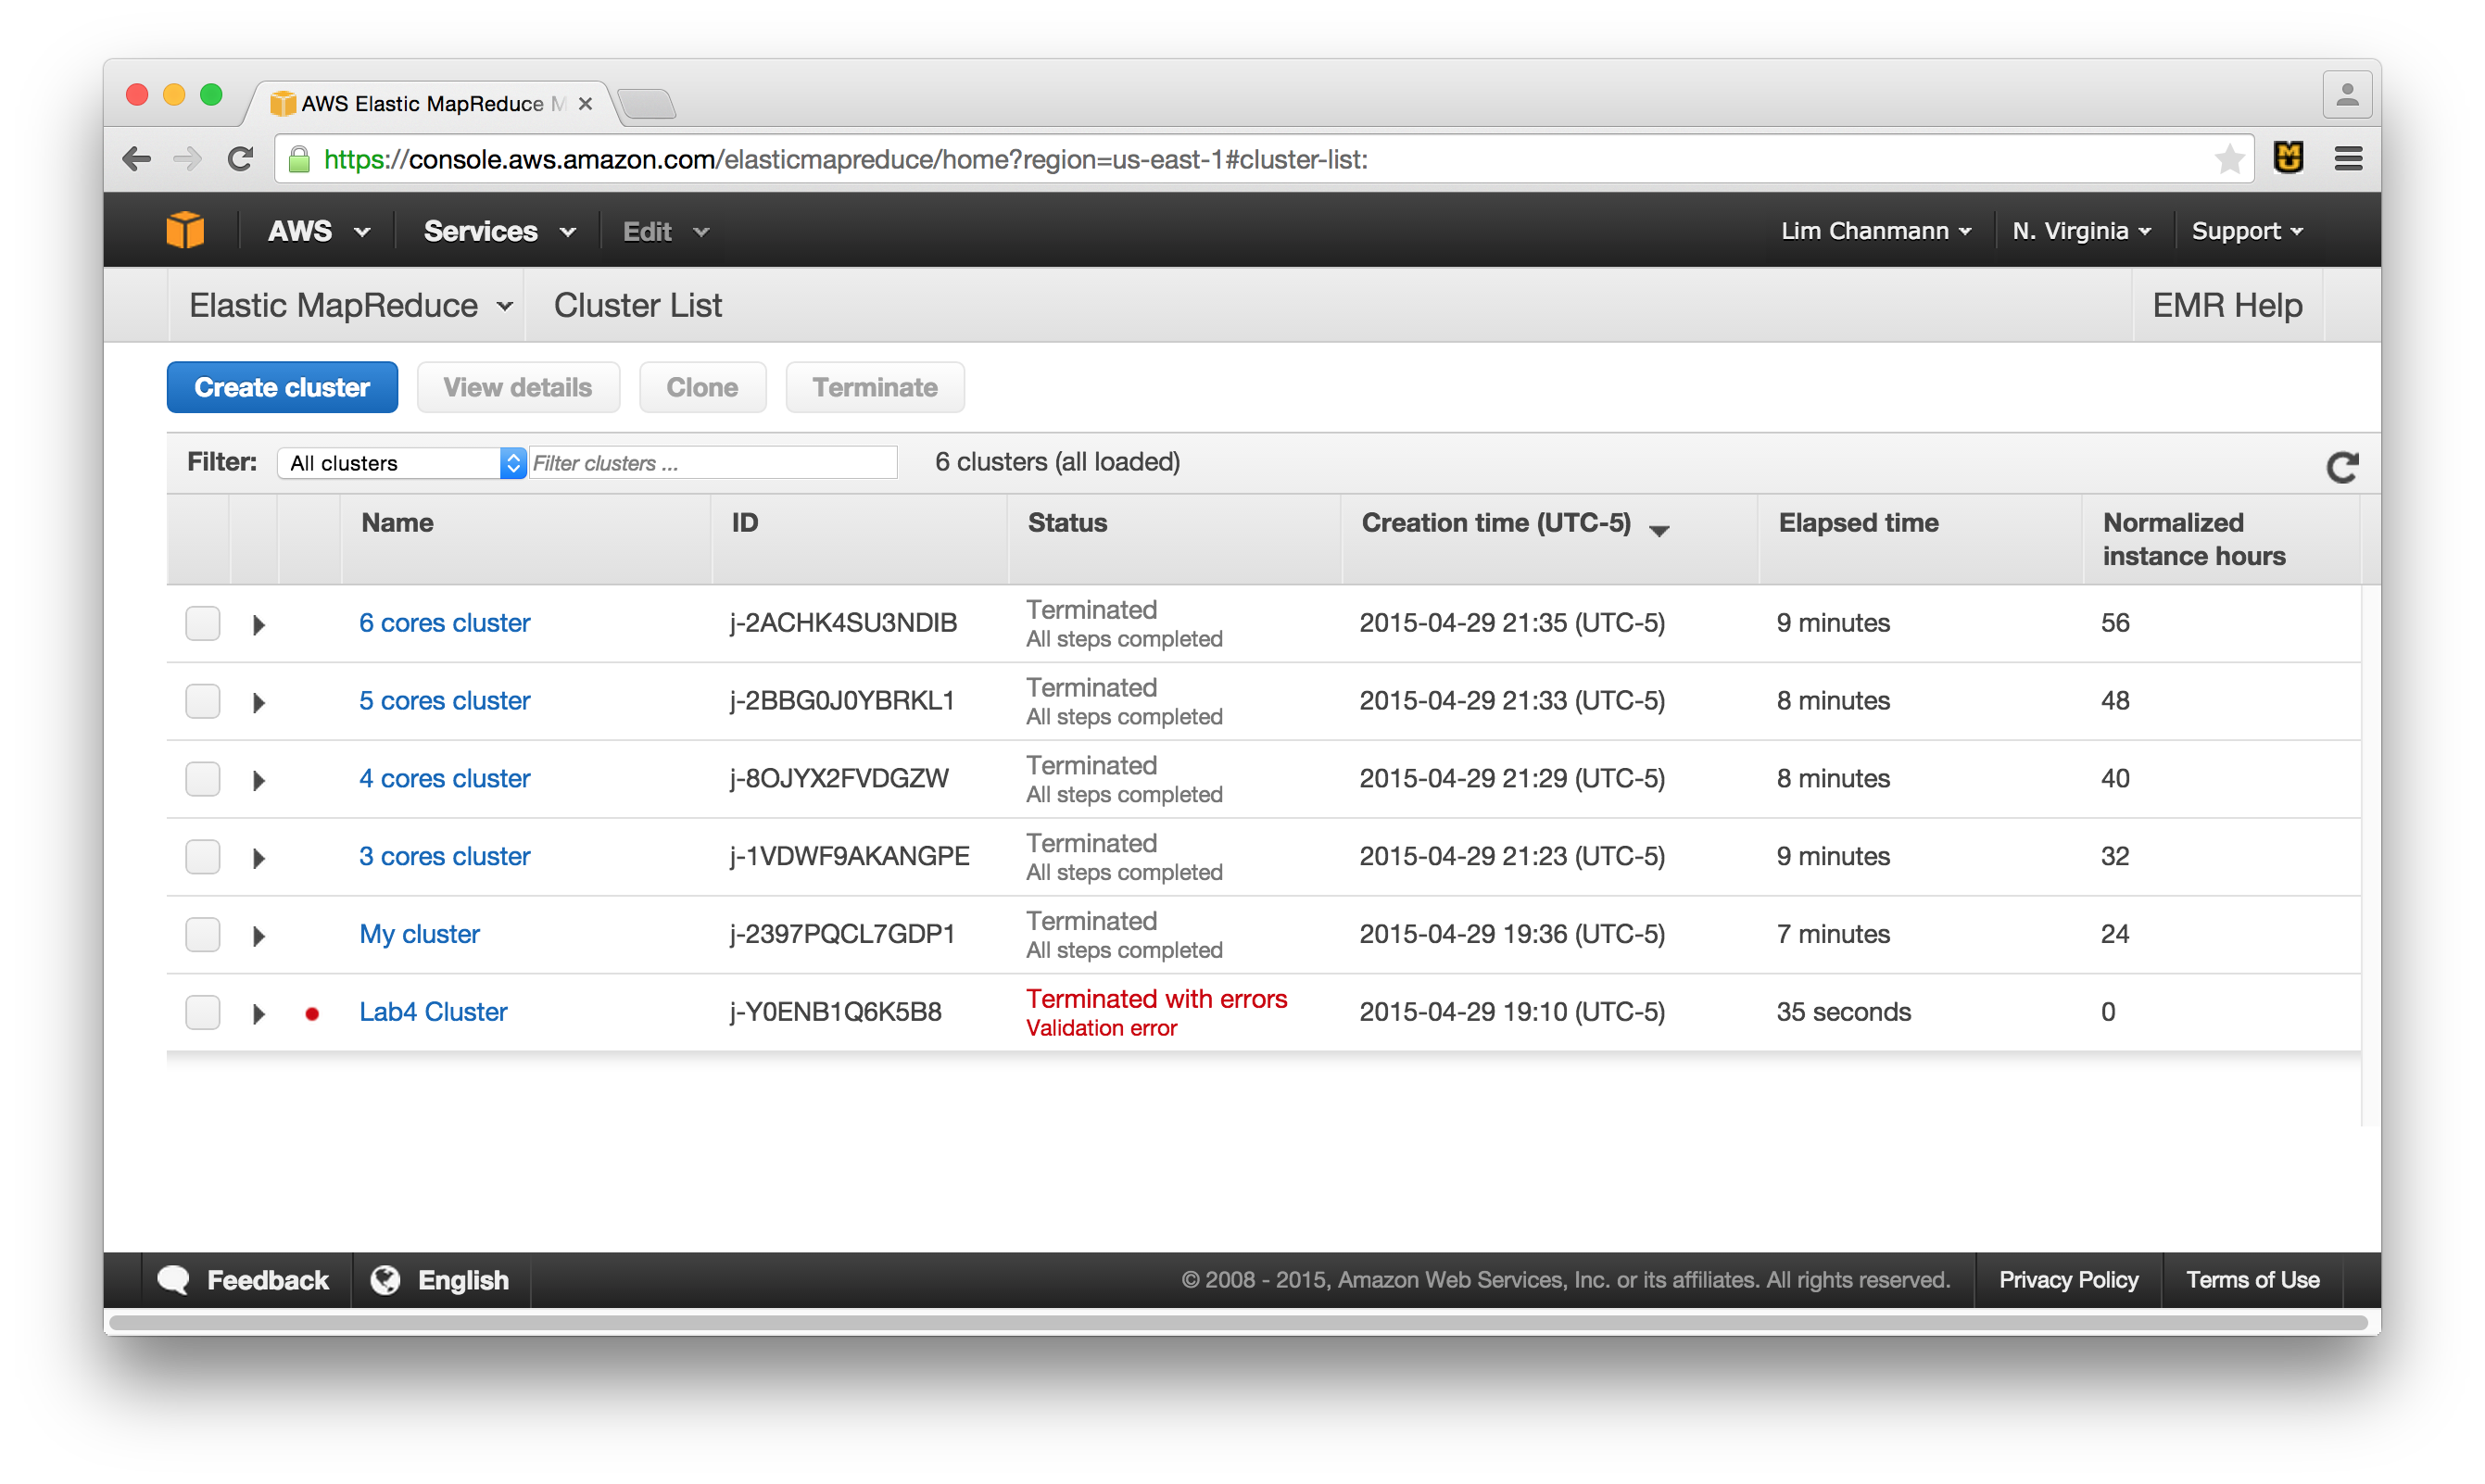
\includegraphics[scale=.37]{emr_clusters.png}
  \caption{Amazon EMR clusters}
\end{figure}


\end{document}